\cleardoublepage
\chapter{RINCIAN HASIL SURVEI ANALISIS KONDISI SAAT INI DAN ANALISIS KEBUTUHAN PENGGUNA (MODUL \emph{PEOPLE-TO-PROJECT})}
\label{chap:lampiran-a}

\section{Instrumen Survei}

Survei disusun dalam dua bagian besar, yaitu bagian umum mengenai profil dan pola partisipasi kolaborasi mahasiswa yang digunakan bersama oleh ketiga modul (\emph{People-to-People}, \emph{People-to-Project}, dan \emph{Team Formation}), dan bagian khusus mengenai kesulitan menilai kecocokan diri serta faktor-faktor yang dianggap penting dalam menentukan kecocokan kegiatan kolaboratif, yang menjadi dasar analisis kebutuhan modul \emph{People-to-Project}. Pertanyaan untuk bagian umum ditunjukkan pada Tabel~\ref{tab:a1-umum}.

\begin{longtable}{p{0.5cm} p{4.5cm} p{2.5cm} p{4.8cm}}
  \caption{Bagian Umum, Profil, dan Partisipasi Kolaborasi (Pertanyaan Bersama)}
  \label{tab:a1-umum} \\
  \toprule
  \textbf{No} & \textbf{Pertanyaan} & \textbf{Tipe} & \textbf{Pilihan Jawaban} \\
  \midrule
  \endfirsthead
  \multicolumn{4}{l}{\small\textit{\tablename~\thetable~(lanjutan)}} \\
  \toprule
  \textbf{No} & \textbf{Pertanyaan} & \textbf{Tipe} & \textbf{Pilihan Jawaban} \\
  \midrule
  \endhead
  \bottomrule
  \multicolumn{4}{r}{\textit{Bersambung ke halaman berikutnya.}} \\
  \endfoot
  \bottomrule
  \endlastfoot
  1 & Pernyataan persetujuan responden & Pilihan tunggal & Saya menyetujui syarat dan ketentuan di atas \\[4pt]
  2 & Program studi Anda saat ini? & Isian singkat & Program studi masing-masing \\[4pt]
  3 & Anda saat ini berada di semester berapa? & Pilihan tunggal & 1--2, 3--4, 5--6, 7--8 \\[4pt]
  4 & Jenis kelamin atau gender Anda? & Pilihan tunggal & Laki-laki, Perempuan \\[4pt]
  5 & Seberapa sering Anda terlibat dalam kegiatan kolaboratif (lomba, proyek, organisasi, dsb.)? & Skala 1--5 & 1 = Tidak pernah, 5 = Sangat sering \\[4pt]
  6 & Jenis kegiatan kolaboratif apa saja yang pernah Anda ikuti? & \emph{Multi-select} & Organisasi, Lomba berkelompok, Proyek inovasi, Proyek bisnis/\emph{startup}, Riset bersama \\
\end{longtable}

Pertanyaan untuk bagian khusus mengenai kesulitan menilai kecocokan diri dan faktor penentu kecocokan kegiatan kolaboratif ditunjukkan pada Tabel~\ref{tab:a2-kecocokan}.

\begin{longtable}{p{0.5cm} p{4.5cm} p{2.5cm} p{4.8cm}}
  \caption{Kesulitan Menilai Kecocokan Diri dan Faktor Penentu Kecocokan Kegiatan Kolaboratif}
  \label{tab:a2-kecocokan} \\
  \toprule
  \textbf{No} & \textbf{Pertanyaan} & \textbf{Tipe} & \textbf{Pilihan Jawaban} \\
  \midrule
  \endfirsthead
  \multicolumn{4}{l}{\small\textit{\tablename~\thetable~(lanjutan)}} \\
  \toprule
  \textbf{No} & \textbf{Pertanyaan} & \textbf{Tipe} & \textbf{Pilihan Jawaban} \\
  \midrule
  \endhead
  \bottomrule
  \multicolumn{4}{r}{\textit{Bersambung ke halaman berikutnya.}} \\
  \endfoot
  \bottomrule
  \endlastfoot
  1 & Bagaimana Anda biasanya menemukan informasi mengenai proyek atau kegiatan kolaboratif? & \emph{Multi-select} & Media Sosial; \emph{Group Chat} (WhatsApp, Line, dan lainnya); Teman atau Kenalan; Dosen; \emph{Platform} Khusus; Lainnya \\[4pt]
  2 & Seberapa sering Anda merasa kesulitan menemukan kegiatan kolaboratif yang sesuai dengan keinginan Anda? & Skala 1--5 & 1 = Sangat jarang, 5 = Sangat sering \\[4pt]
  3 & Apa yang paling menyulitkan Anda dalam mencari kegiatan kolaboratif? & \emph{Multi-select} & Informasi proyek tidak terpusat; Tidak adanya \emph{platform} khusus; Tidak mengetahui apakah kemampuan sesuai; Tidak memahami peran apa yang dibutuhkan; Kurangnya rekomendasi atau saran; Lainnya \\[4pt]
  4 & Seberapa Anda membutuhkan bantuan dalam menentukan kegiatan kolaboratif yang sesuai bagi Anda (terkhusus bagi mahasiswa)? & Skala 1--5 & 1 = Tidak butuh, 5 = Sangat butuh \\[4pt]
  5 & Menurut Anda, apa faktor terpenting dalam menentukan kecocokan kegiatan kolaboratif dengan Anda? & \emph{Multi-select} & Minat pribadi; Kemampuan/\emph{skill}; Pengalaman sebelumnya; Preferensi peran; Ketersediaan waktu; \emph{Work Style}; Lainnya \\[4pt]
  6 & Seberapa setuju Anda bahwa sistem yang dapat menilai kecocokan kegiatan kolaboratif berdasarkan profil (minat, \emph{skill}, dsb.) akan dapat membantu? & Skala 1--5 & 1 = Sangat tidak setuju, 5 = Sangat setuju \\[4pt]
  7 & Jika terdapat \emph{platform} rekomendasi kegiatan kolaboratif berbasis kecocokan profil (khusus mahasiswa), apakah Anda tertarik menggunakannya? & Skala 1--5 & 1 = Sangat tidak tertarik, 5 = Sangat tertarik \\[4pt]
  8 & Menurut Anda, apakah \emph{platform} seperti ini dapat mempermudah Anda dalam mengambil keputusan terkait memilih kegiatan kolaboratif? & Skala 1--5 & 1 = Sangat tidak mempermudah, 5 = Sangat mempermudah \\
\end{longtable}

Catatan: opsi jawaban pada Tabel~\ref{tab:a2-kecocokan} ditulis mengikuti label asli pada instrumen kuesioner (misalnya \emph{Work Style} dan \emph{Preferensi role}), sedangkan narasi pada Bab III dan Bab IV menggunakan istilah terjemahan ``gaya kerja'' dan ``preferensi peran'' untuk konsistensi bahasa laporan.

\section{Metodologi Survei}

Survei ini melibatkan 86 mahasiswa aktif dari berbagai program studi dan tingkat semester sebagai populasi/sampel penelitian. Teknik pengambilan sampel yang digunakan bersifat \emph{voluntary/convenience sampling}, yaitu responden mengisi kuesioner secara sukarela berdasarkan kemudahan akses penyebaran. Meskipun tidak menggunakan teknik \emph{sampling} probabilistik, jumlah responden tersebut dinilai cukup memadai untuk memberikan gambaran awal mengenai pola perilaku, hambatan, serta kebutuhan mahasiswa dalam proses pencarian kegiatan kolaboratif. Instrumen yang digunakan dalam survei ini berupa kuesioner daring melalui Google Form. Kuesioner disebarkan melalui berbagai kanal komunikasi mahasiswa, seperti grup angkatan, grup kelas, aplikasi \emph{messaging}, serta media sosial sehingga dapat menjangkau responden dari latar program studi dan tingkat semester yang beragam. Cakupan survei ini digunakan bersama oleh tiga modul, yaitu \emph{People-to-People}, \emph{People-to-Project}, dan \emph{Team Formation}, khususnya untuk bagian pertanyaan umum, dengan tambahan pertanyaan spesifik sesuai kebutuhan analisis modul masing-masing.

\section{Hasil Jawaban Survei}

Bagian ini menyajikan ruang untuk visualisasi hasil jawaban responden pada tiap pertanyaan instrumen survei sebagai rincian lengkap dari temuan yang telah dirangkum pada Bab III. Karena bagian umum (Tabel~\ref{tab:a1-umum}) merupakan instrumen bersama, hasil pada Gambar~\ref{fig:lampiran-a1} sampai Gambar~\ref{fig:lampiran-a5} identik dengan yang disajikan pada lampiran modul lain, sedangkan Gambar~\ref{fig:lampiran-a6} sampai Gambar~\ref{fig:lampiran-a13} merupakan hasil khusus pertanyaan modul \emph{People-to-Project} (Tabel~\ref{tab:a2-kecocokan}).

\begin{figure}[H]
\centering
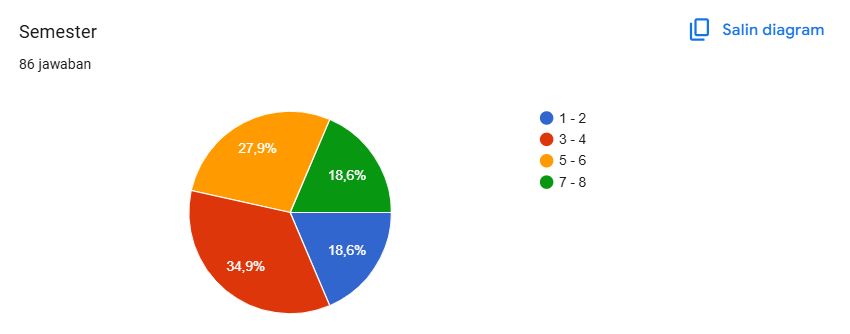
\includegraphics[width=0.85\textwidth]{images/SurveiAwal/survei1.png}
\caption{Distribusi semester responden}
\label{fig:lampiran-a1}
\end{figure}

\begin{figure}[H]
\centering
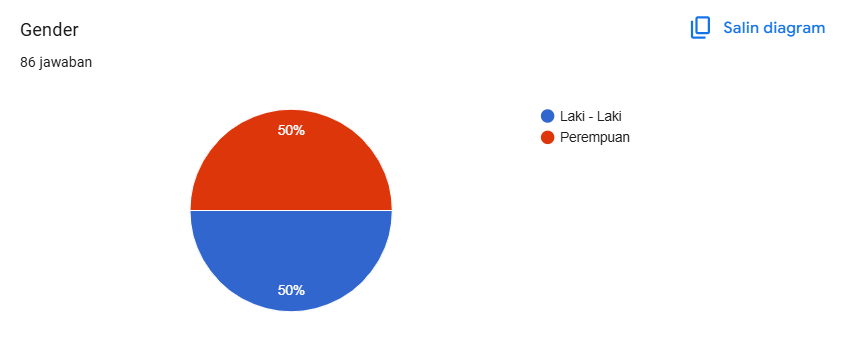
\includegraphics[width=0.85\textwidth]{images/SurveiAwal/survei2.png}
\caption{Distribusi jenis kelamin atau gender responden}
\label{fig:lampiran-a2}
\end{figure}

\begin{figure}[H]
\centering
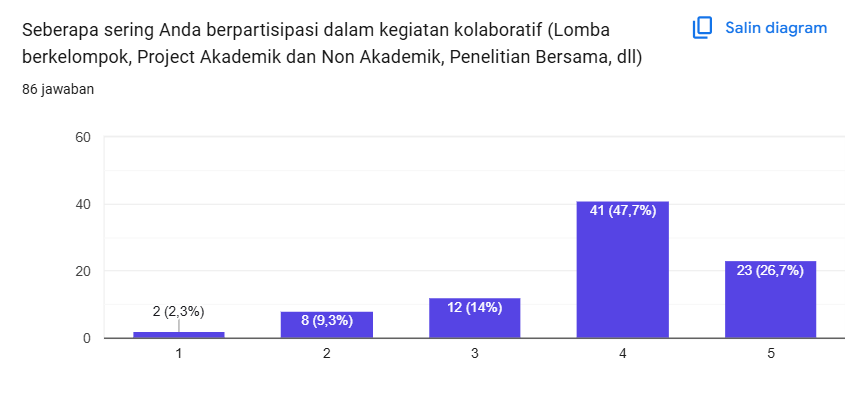
\includegraphics[width=0.85\textwidth]{images/SurveiAwal/survei3.png}
\caption{Tingkat keterlibatan responden dalam kegiatan kolaboratif}
\label{fig:lampiran-a3}
\end{figure}

\begin{figure}[H]
\centering
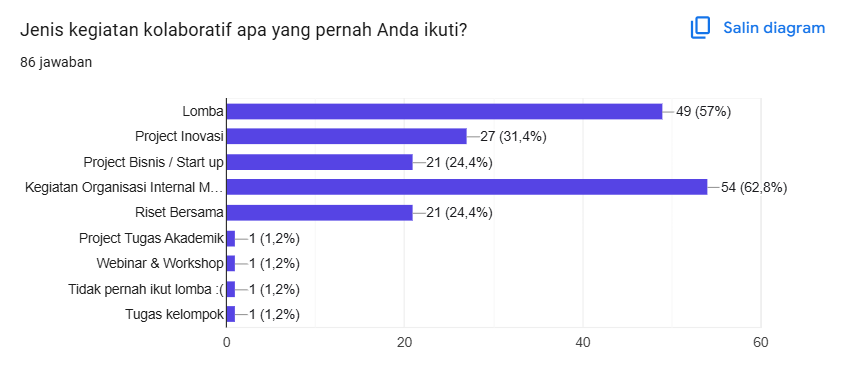
\includegraphics[width=0.85\textwidth]{images/SurveiAwal/survei4.png}
\caption{Jenis kegiatan kolaboratif yang pernah diikuti responden}
\label{fig:lampiran-a4}
\end{figure}

\begin{figure}[H]
\centering
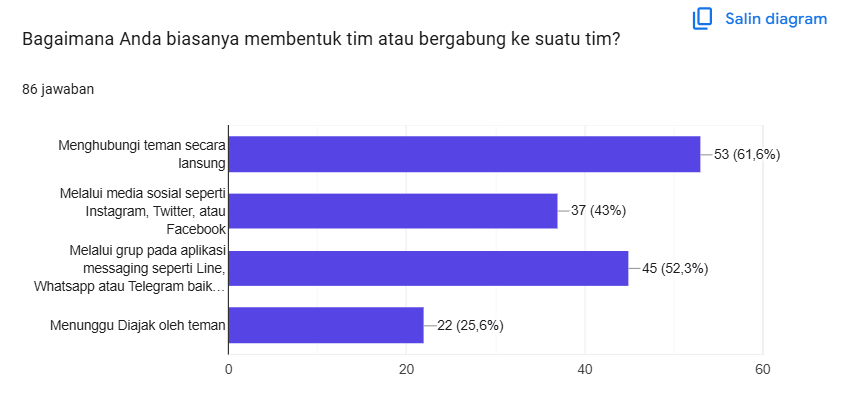
\includegraphics[width=0.85\textwidth]{images/SurveiAwal/survei5.png}
\caption{Distribusi program studi responden}
\label{fig:lampiran-a5}
\end{figure}

\begin{figure}[H]
\centering
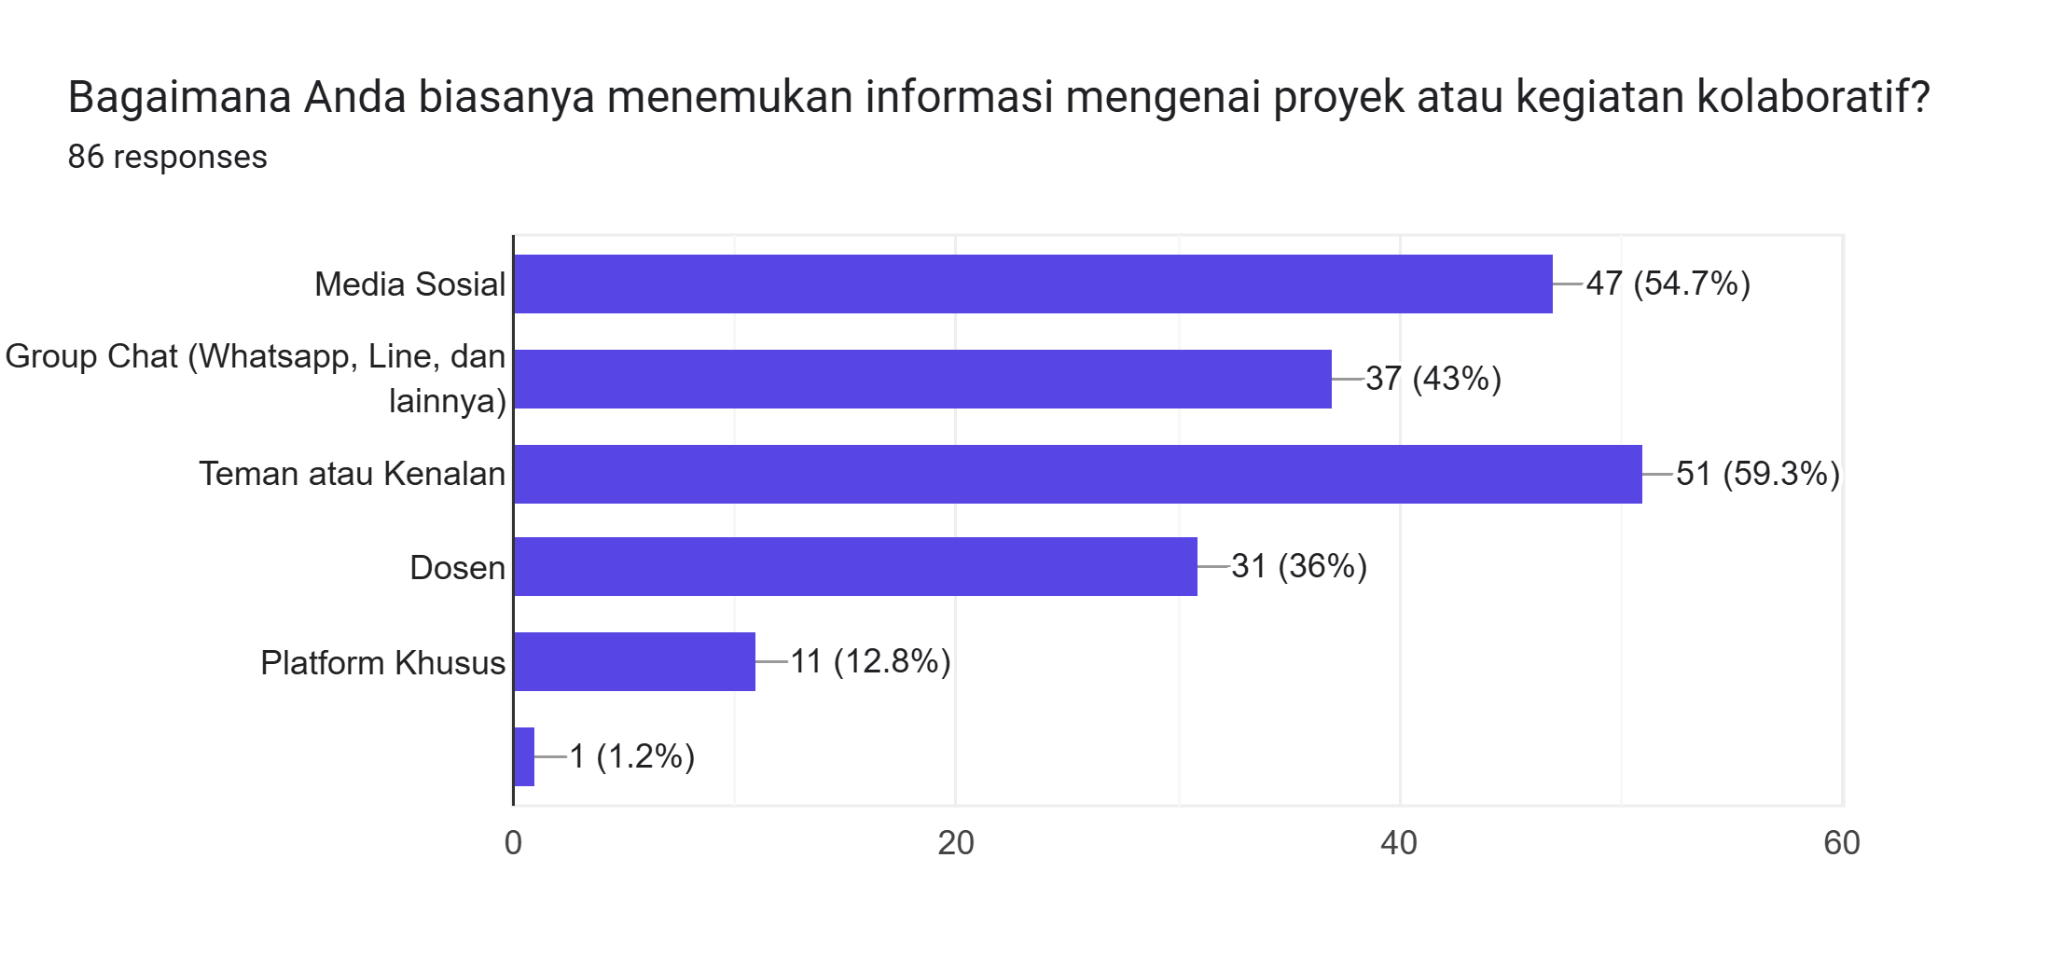
\includegraphics[width=0.85\textwidth]{images/SurveiAwal/survei6.png}
\caption{Cara responden menemukan informasi mengenai proyek atau kegiatan kolaboratif}
\label{fig:lampiran-a6}
\end{figure}

\begin{figure}[H]
\centering
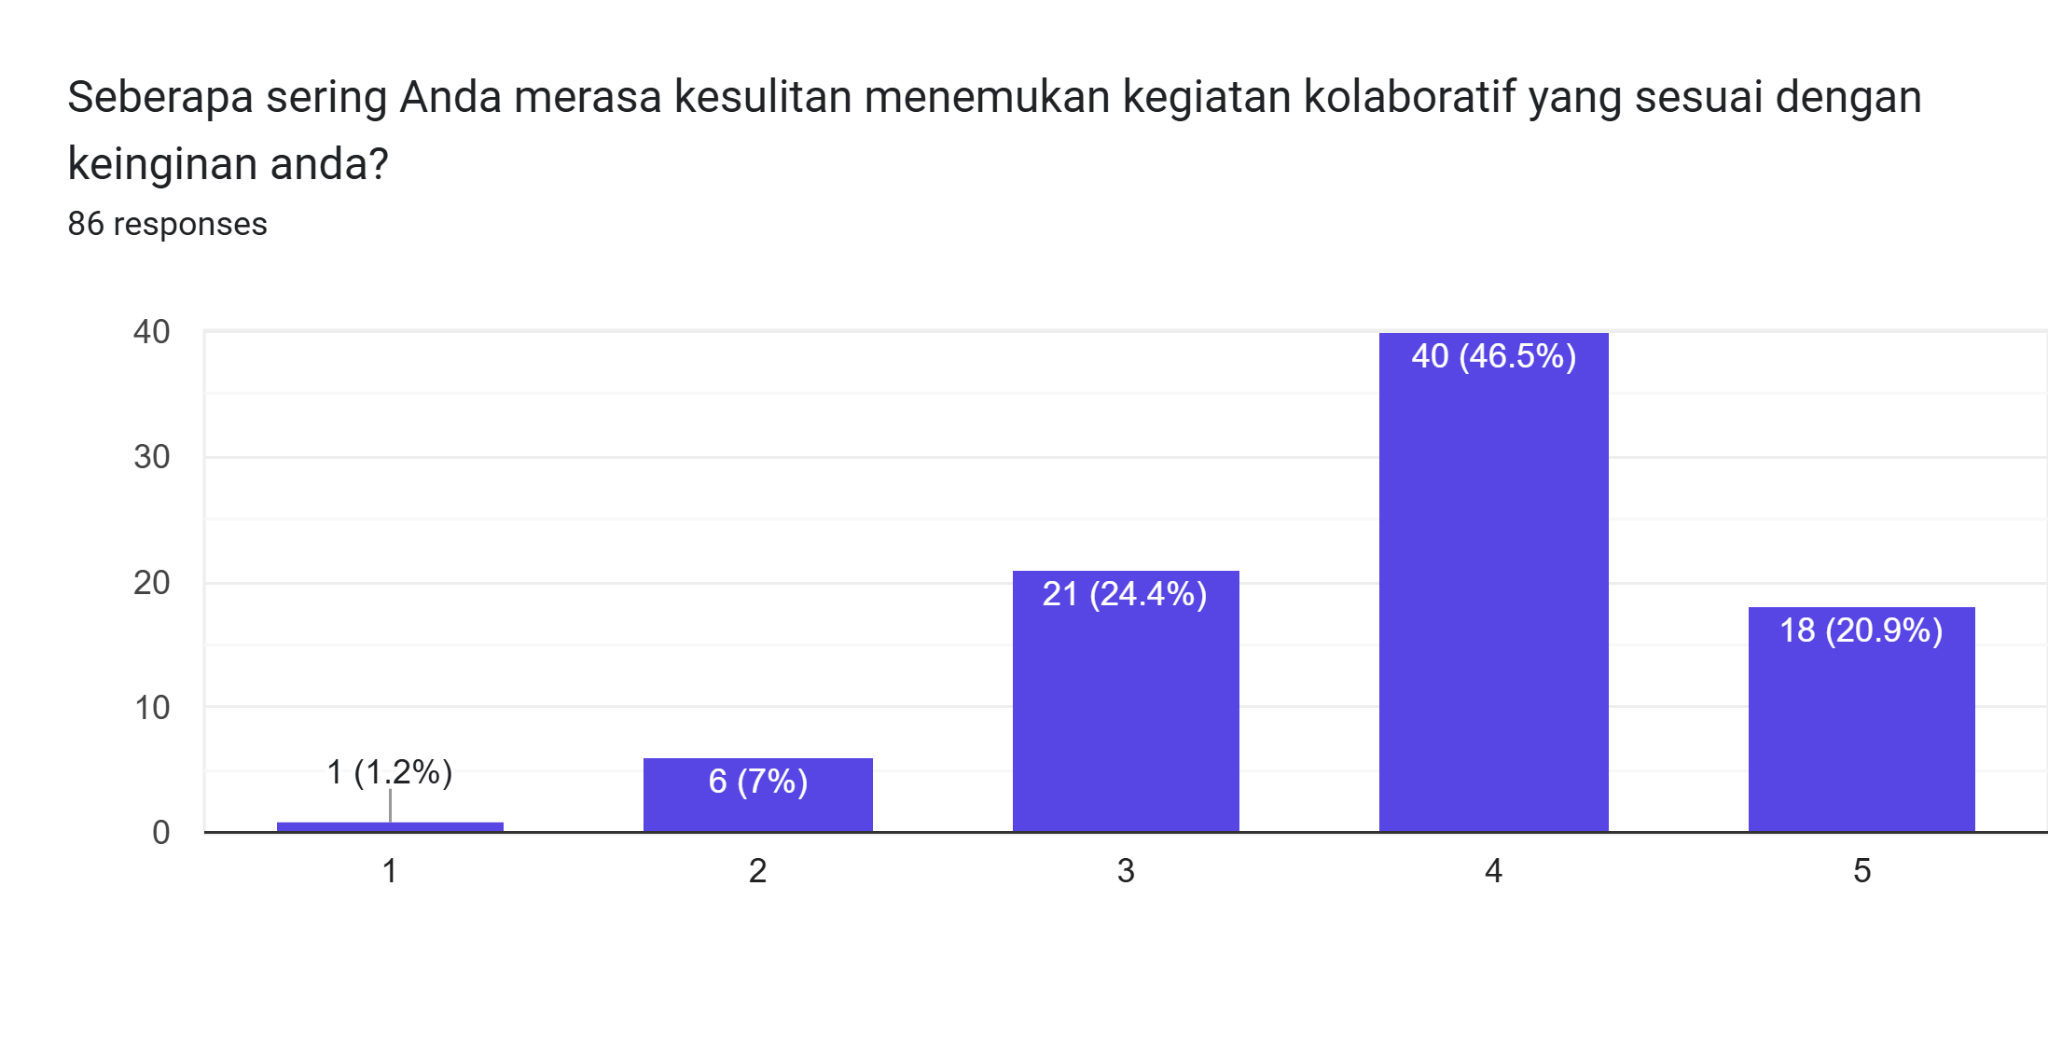
\includegraphics[width=0.85\textwidth]{images/SurveiAwal/survei7.png}
\caption{Tingkat kesulitan responden menemukan kegiatan kolaboratif yang sesuai dengan keinginan}
\label{fig:lampiran-a7}
\end{figure}

\begin{figure}[H]
\centering
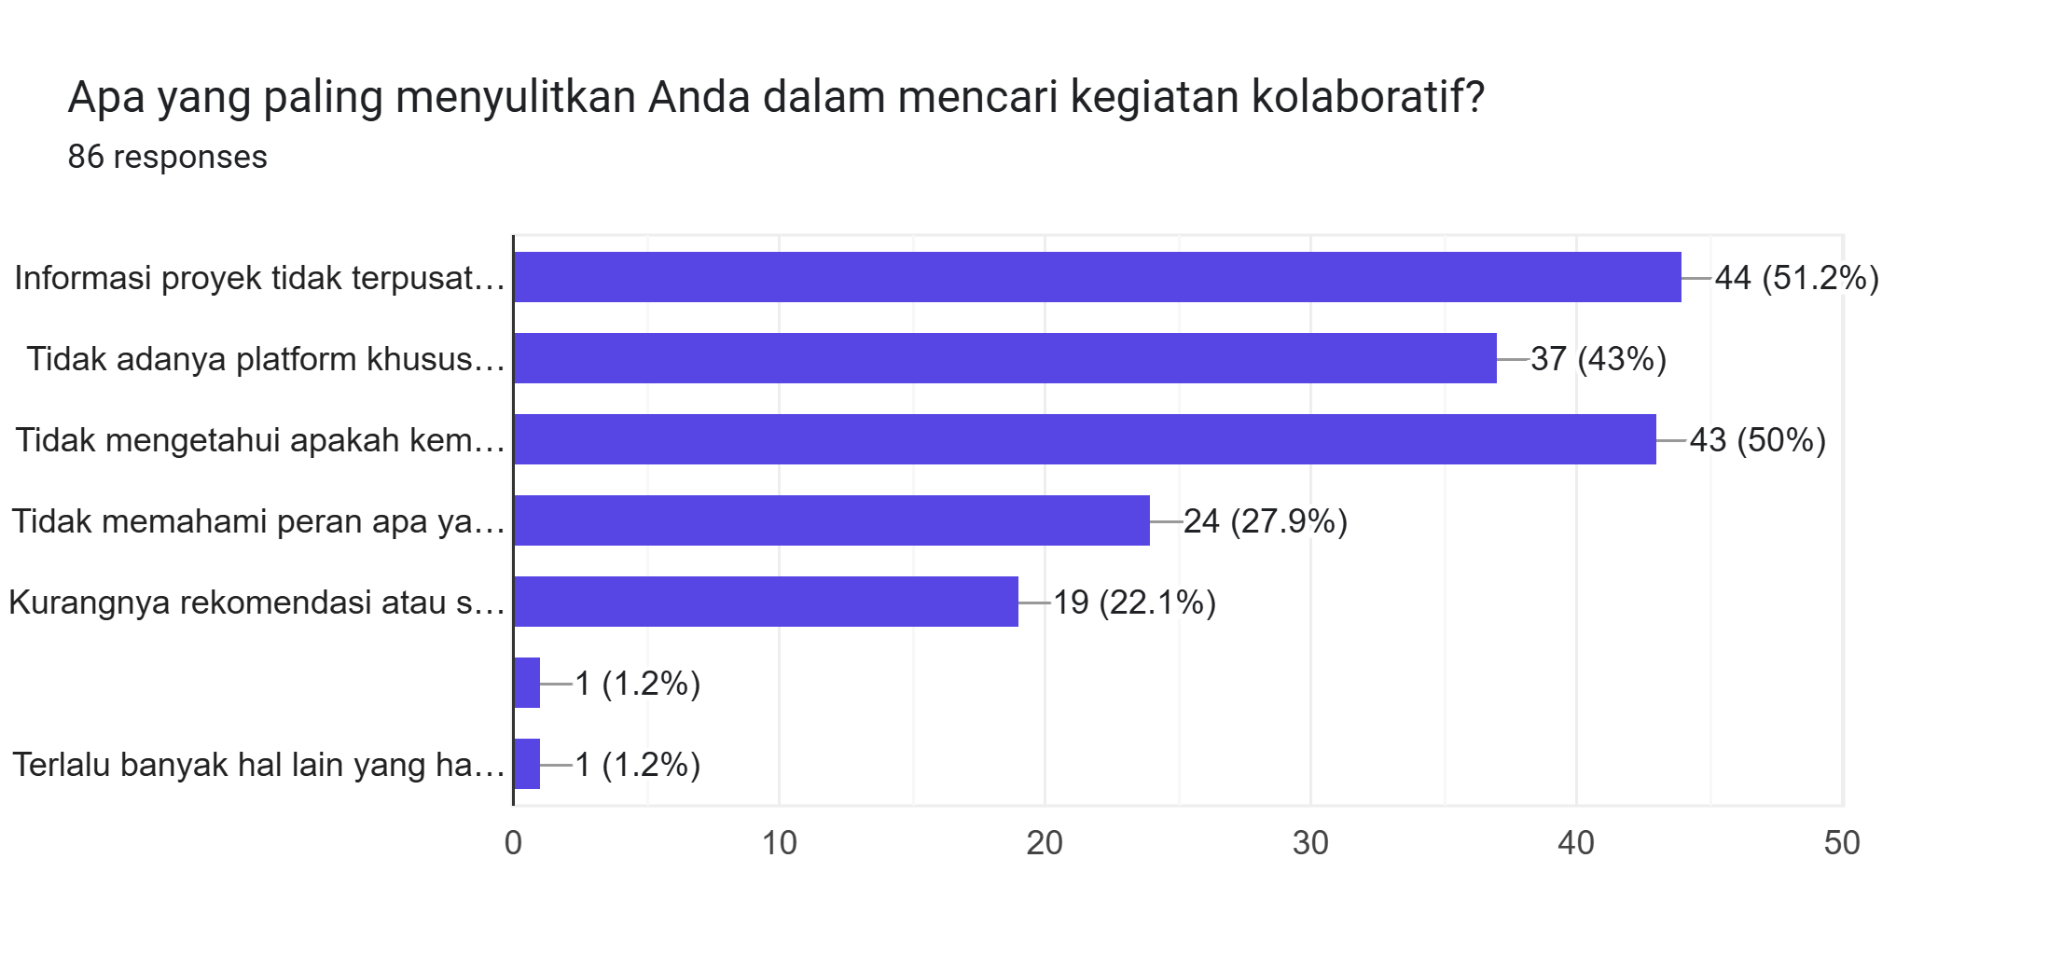
\includegraphics[width=0.85\textwidth]{images/SurveiAwal/survei8.png}
\caption{Hal yang paling menyulitkan responden dalam mencari kegiatan kolaboratif}
\label{fig:lampiran-a8}
\end{figure}

\begin{figure}[H]
\centering
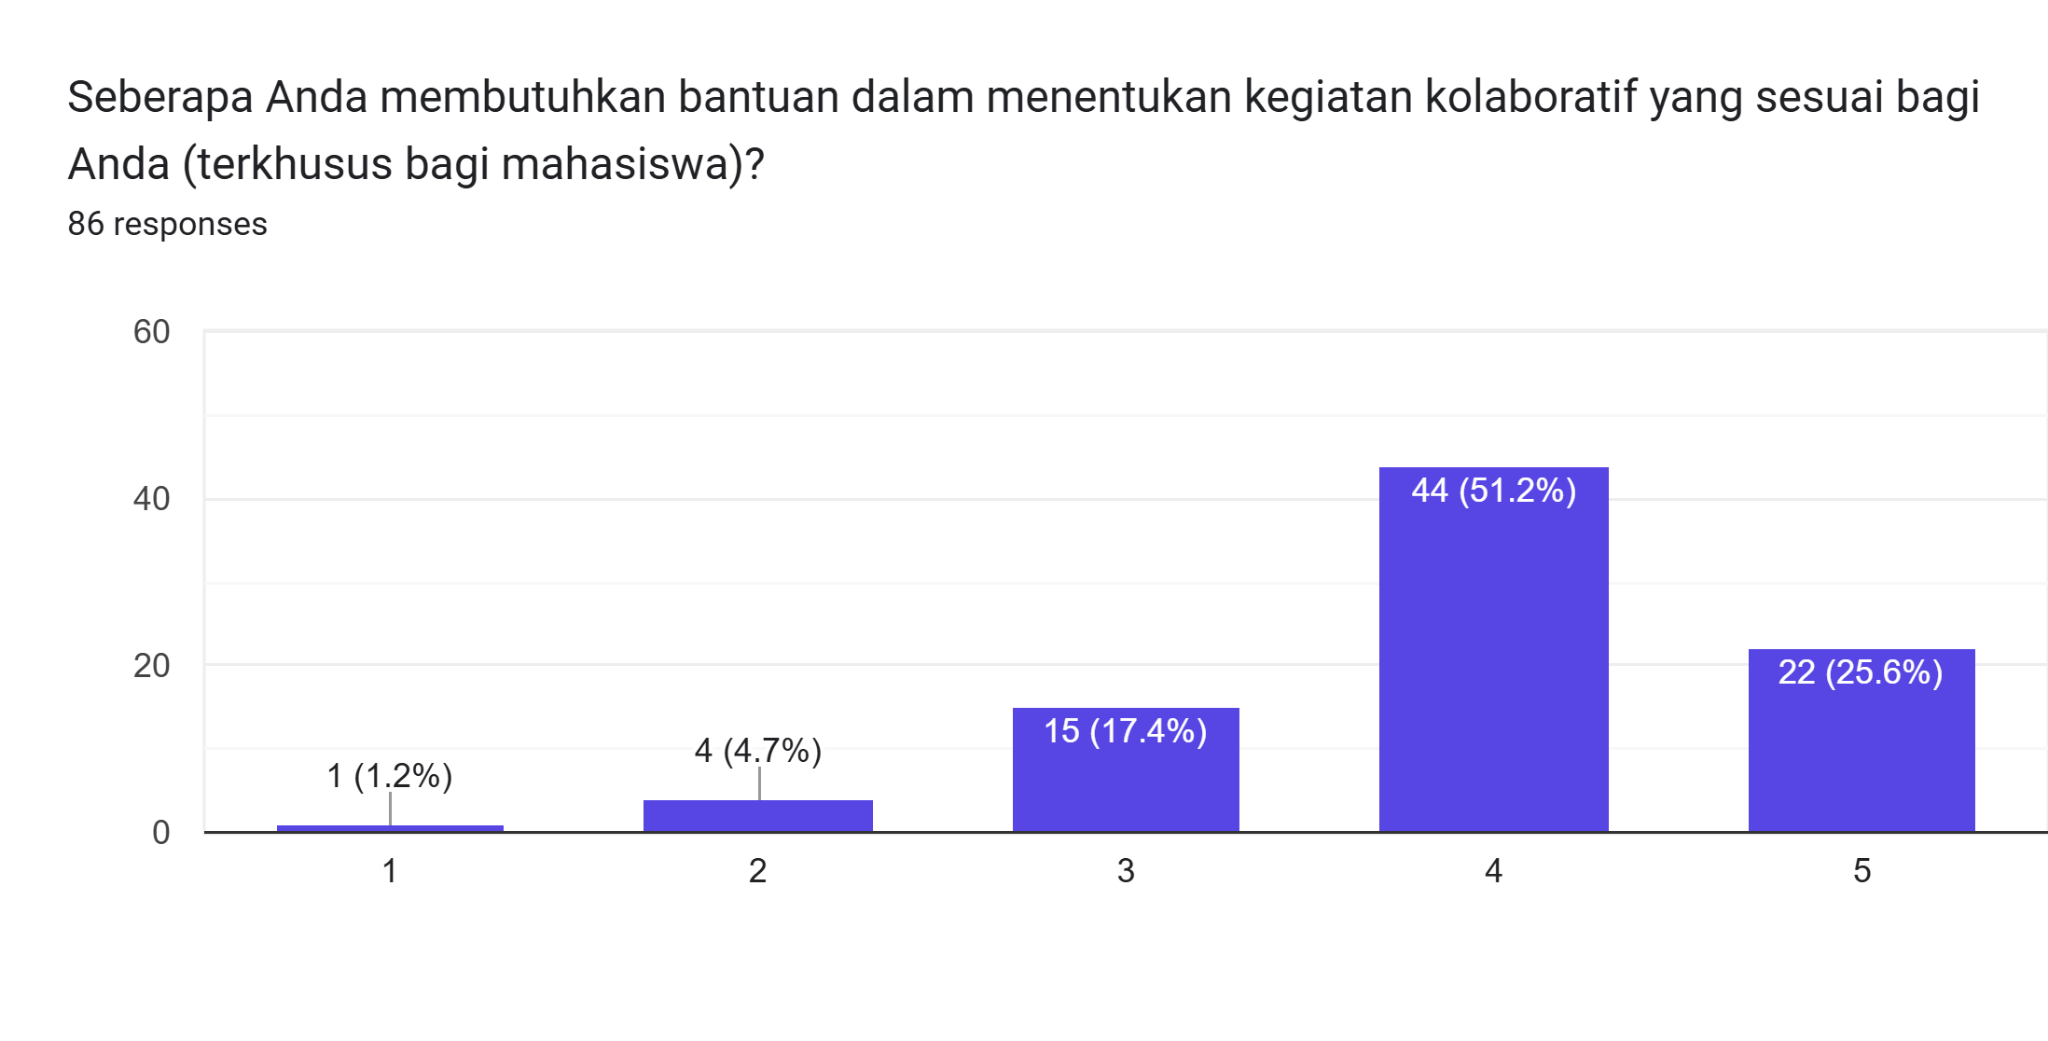
\includegraphics[width=0.85\textwidth]{images/SurveiAwal/survei9.png}
\caption{Tingkat kebutuhan responden akan bantuan dalam menentukan kegiatan kolaboratif yang sesuai}
\label{fig:lampiran-a9}
\end{figure}

\begin{figure}[H]
\centering
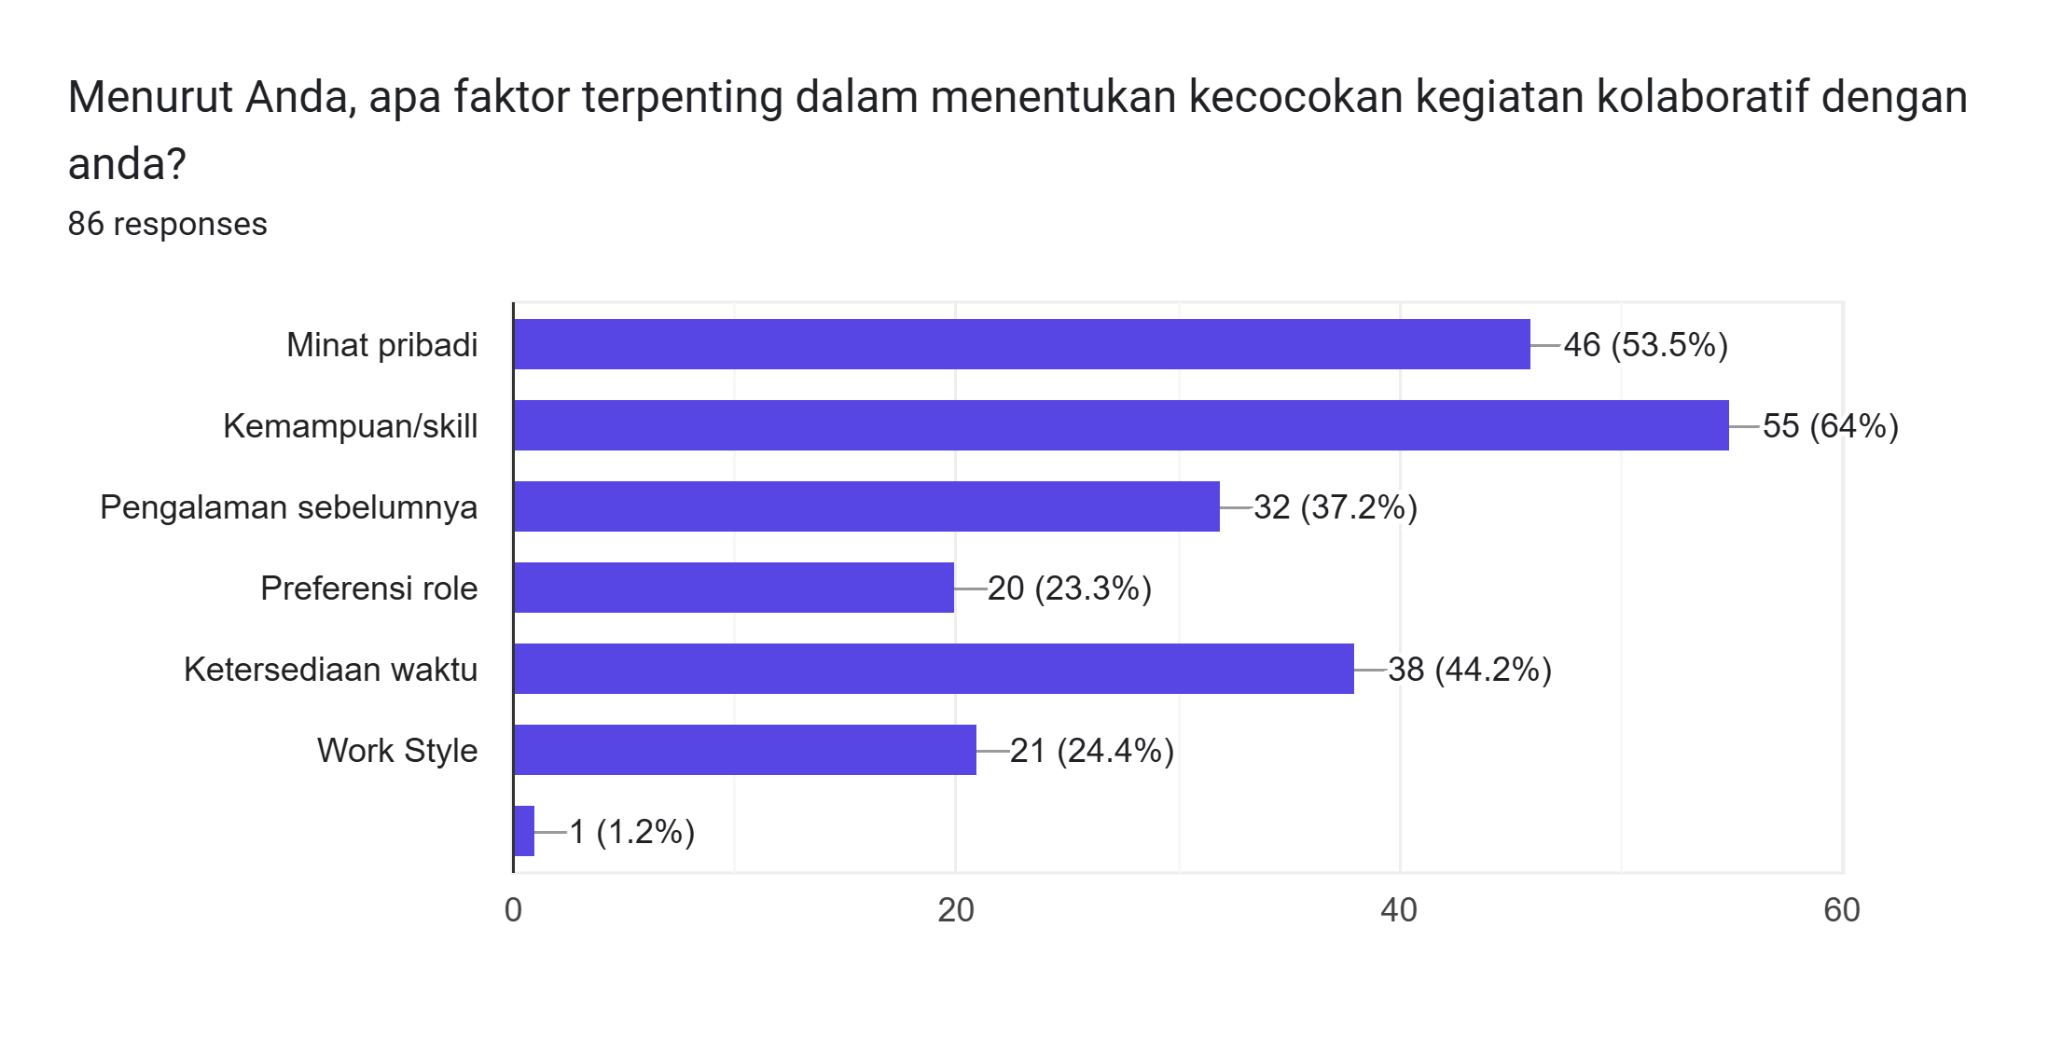
\includegraphics[width=0.85\textwidth]{images/SurveiAwal/survei10.png}
\caption{Faktor yang dianggap terpenting dalam menentukan kecocokan kegiatan kolaboratif menurut responden}
\label{fig:lampiran-a10}
\end{figure}

\begin{figure}[H]
\centering
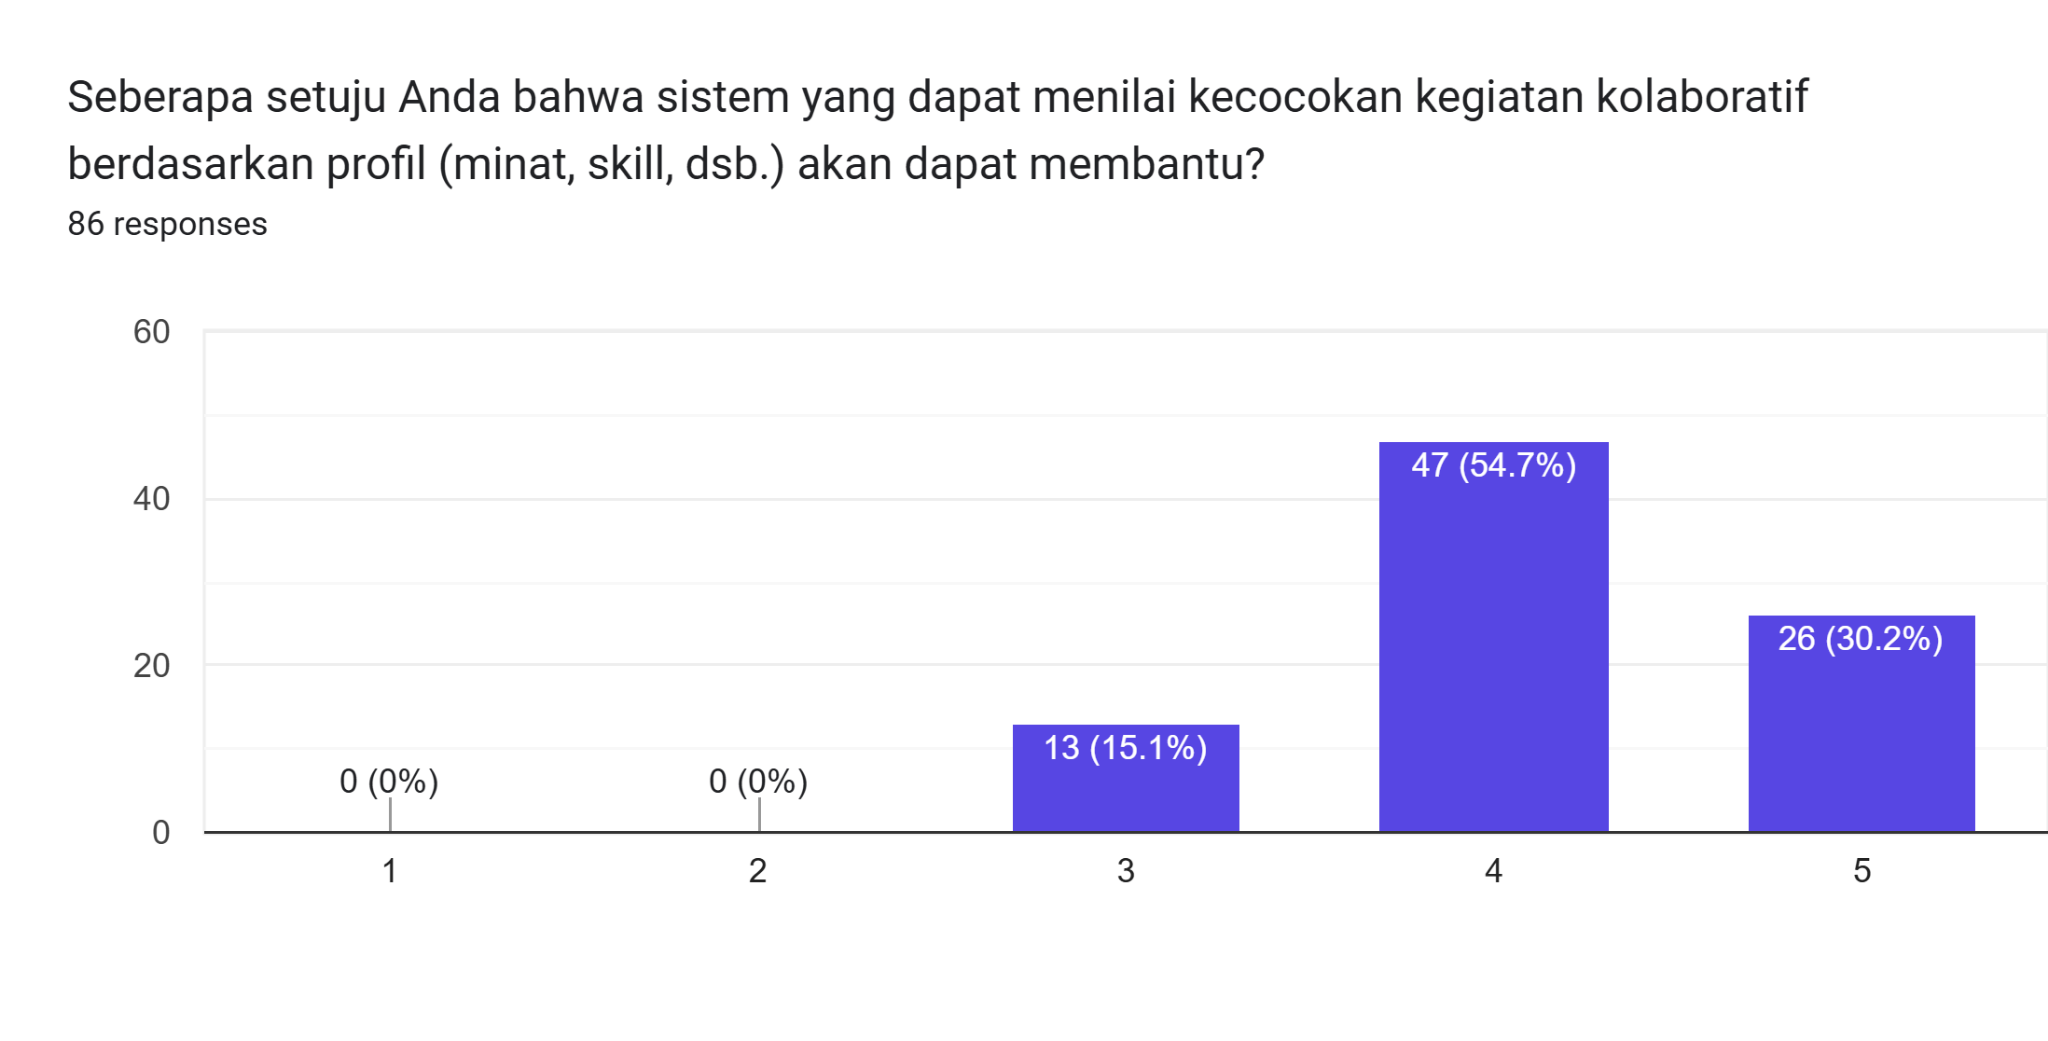
\includegraphics[width=0.85\textwidth]{images/SurveiAwal/survei11.png}
\caption{Tingkat kesetujuan responden bahwa sistem penilai kecocokan berdasarkan profil akan membantu}
\label{fig:lampiran-a11}
\end{figure}

\begin{figure}[H]
\centering
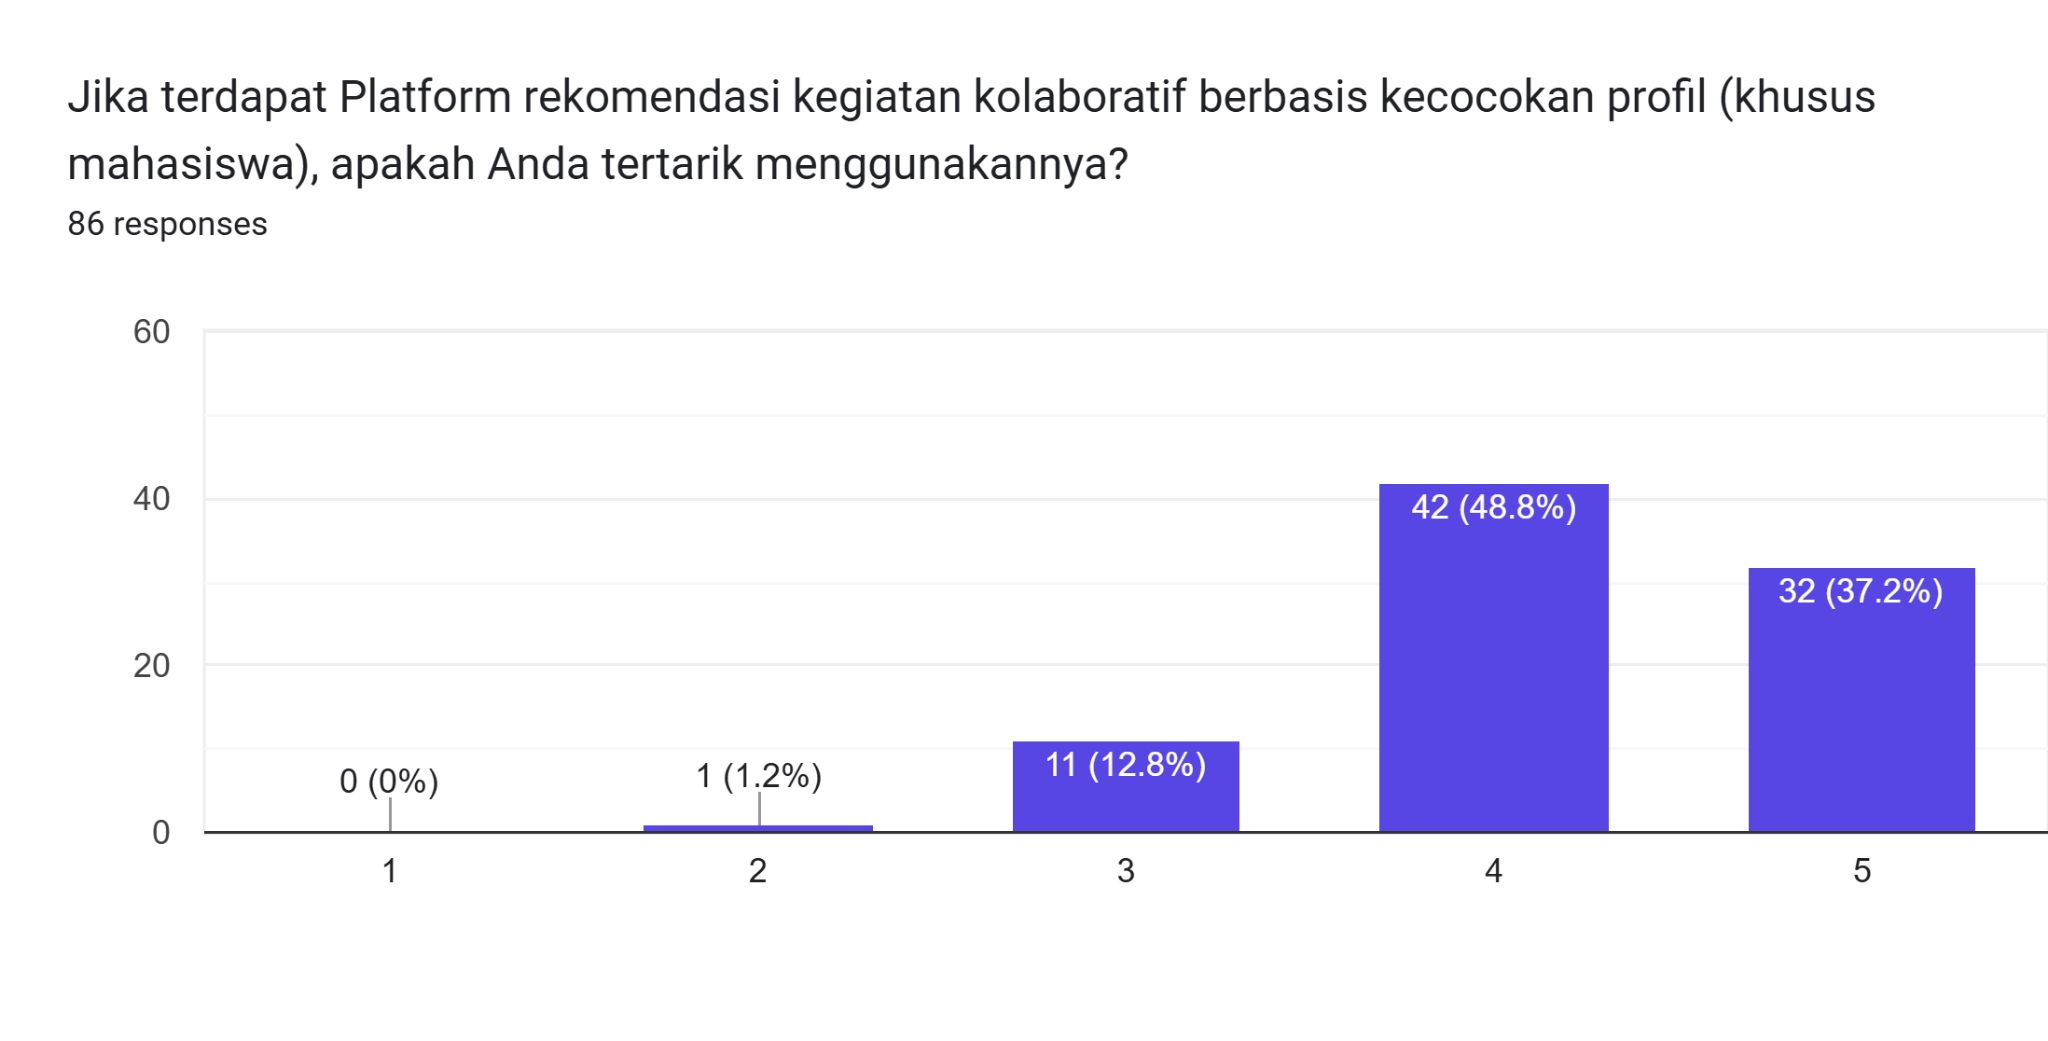
\includegraphics[width=0.85\textwidth]{images/SurveiAwal/survei12.png}
\caption{Tingkat ketertarikan responden menggunakan \emph{platform} rekomendasi kegiatan kolaboratif berbasis kecocokan profil}
\label{fig:lampiran-a12}
\end{figure}

\begin{figure}[H]
\centering
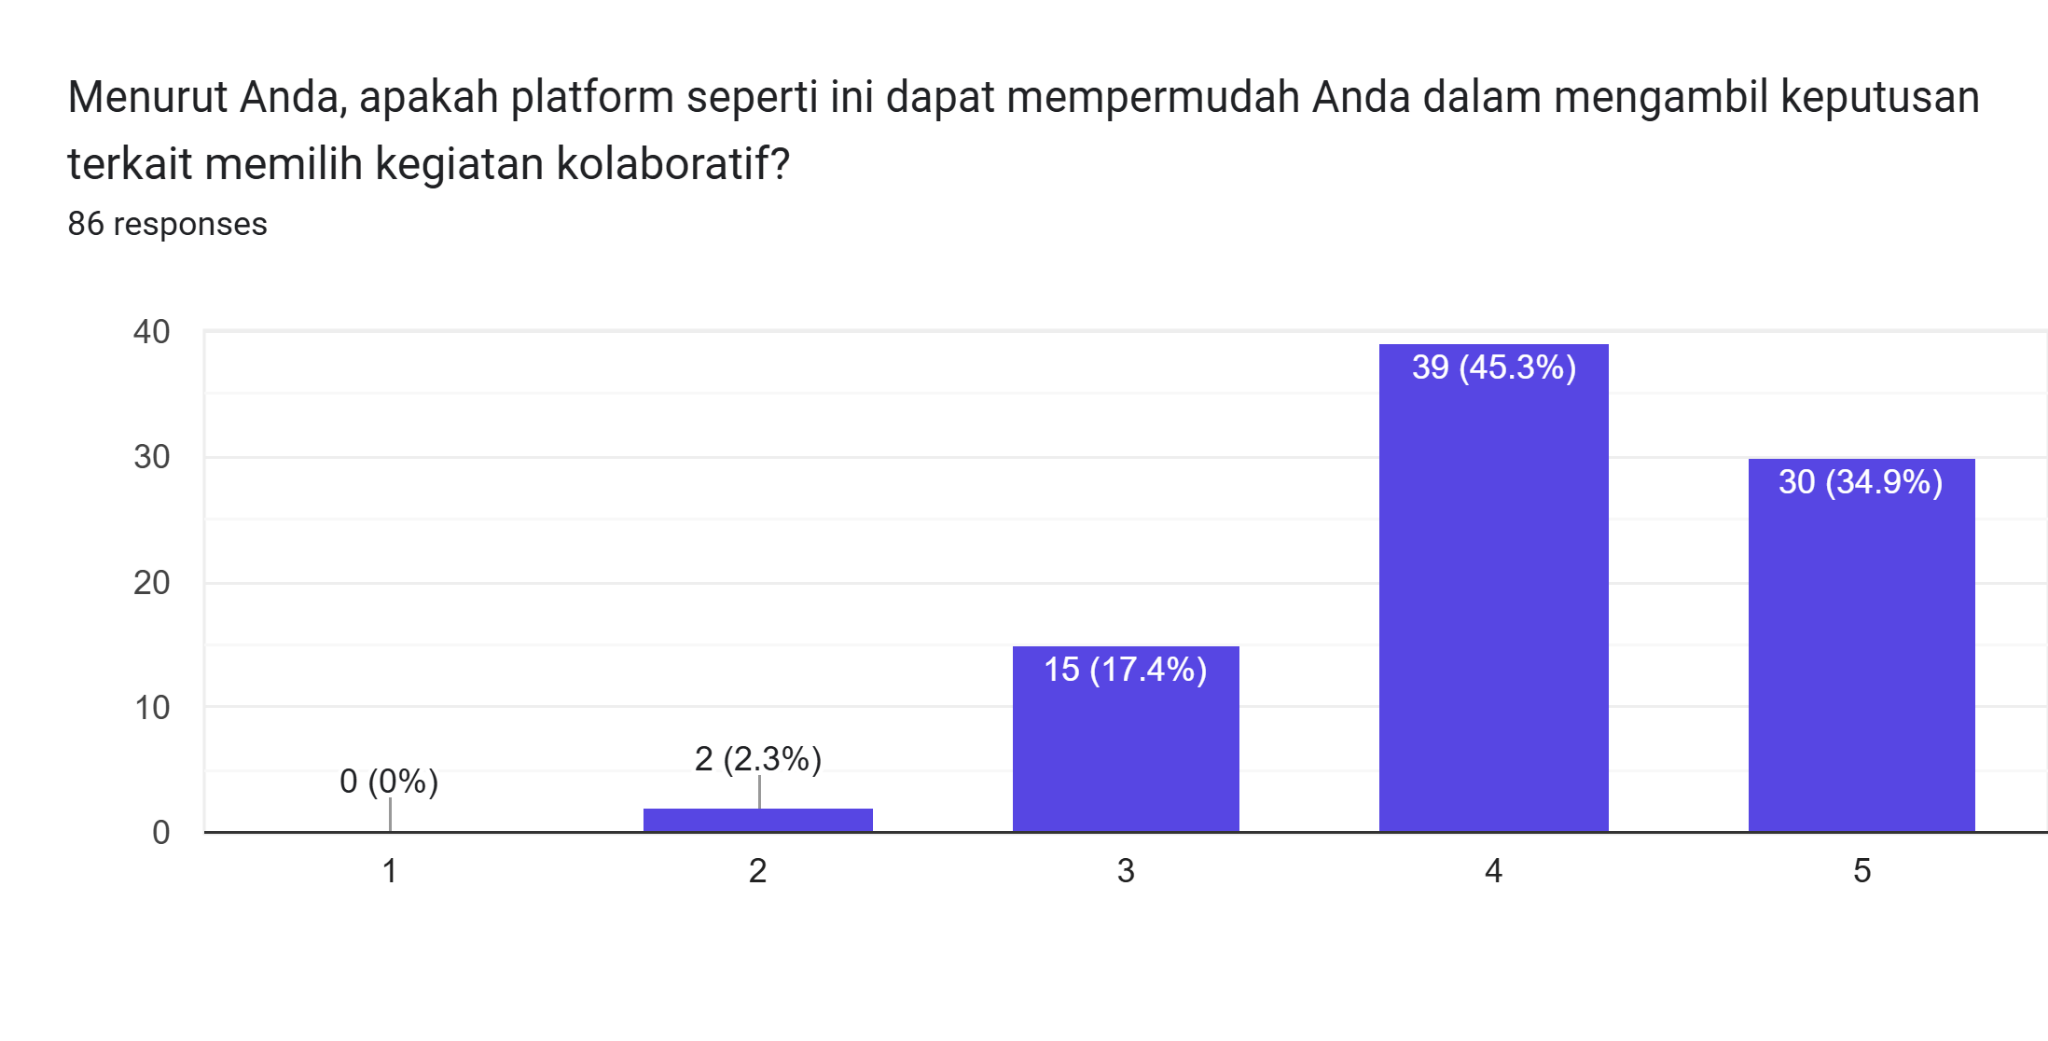
\includegraphics[width=0.85\textwidth]{images/SurveiAwal/survei13.png}
\caption{Tingkat kepercayaan responden bahwa \emph{platform} tersebut dapat mempermudah pengambilan keputusan}
\label{fig:lampiran-a13}
\end{figure}
